\chapter{Trust regions: TRPO and PPO}
\label{ch:ppo}

A2C makes one gradient step per batch of experience and discards the
batch. Making several steps on the same batch would use the data better,
but after the first step the batch was generated by an older policy, and a
large step can ruin a policy that took millions of games to learn. This
chapter derives a surrogate objective that is accurate near the current
policy, and the clipping mechanism of proximal policy optimisation (PPO,
Schulman et al., 2017) that keeps the updates within the region where the
surrogate can be trusted. PPO is the algorithm of the best agent of the
repository.

Throughout the chapter, $\pi$ is the current policy (the one that played
the batch) and $\pi'$ a candidate new policy. We use the discounted
objective $J(\pi) = \E_\pi[G_0]$ of \cref{ch:pg}, episodes of bounded length
and finitely many states and actions.

\section{How good is a new policy?}

\begin{lemma}{Performance difference lemma}{perf-diff}
  For any two policies $\pi$ and $\pi'$,
  \begin{equation}
    \label{eq:perf-diff}
    J(\pi') - J(\pi) = \E_{\pi'}\left[ \sum_{t \geq 0} \gamma^t\,
    A_\pi(S_t, A_t) \right],
  \end{equation}
  where the trajectory is generated by $\pi'$ and the advantages are those
  of $\pi$ (Kakade and Langford, 2002).
\end{lemma}

\begin{proof}
  Given $(S_t, A_t)$, $\E[R_{t+1} + \gamma v_\pi(S_{t+1}) \mid S_t, A_t] =
  q_\pi(S_t, A_t)$ whatever the policy that generated the trajectory, since
  this involves only the dynamics. Hence, by the tower property,
  \begin{equation*}
    \E_{\pi'}\left[ \sum_t \gamma^t A_\pi(S_t, A_t) \right]
    = \E_{\pi'}\left[ \sum_t \gamma^t \left( R_{t+1} + \gamma v_\pi(S_{t+1})
      - v_\pi(S_t) \right) \right].
  \end{equation*}
  The sum is finite (bounded episodes, $v_\pi = 0$ at the end), and the
  value terms telescope: $\sum_t \gamma^t (\gamma v_\pi(S_{t+1}) -
  v_\pi(S_t)) = -v_\pi(S_0)$. What remains is $\E_{\pi'}[G_0] -
  \E[v_\pi(S_0)] = J(\pi') - J(\pi)$, the initial distribution being the
  same for both policies.
\end{proof}

\begin{intuition}
  The gain of a new policy is the sum, along its own games, of how much
  better each of its moves is than what the old policy would have done
  on average, as judged by the old policy's own values. It is like
  evaluating a new player's moves with an old coach's judgement: every
  move the coach rates above average adds to the score.
\end{intuition}

The lemma says that $\pi'$ is better than $\pi$ if it plays actions of
positive advantage (for $\pi$) in the states \emph{it} visits. We cannot
evaluate the right-hand side without playing $\pi'$, but we can evaluate
the actions of $\pi'$ on the states visited by $\pi$, using importance
sampling.

\begin{proposition}{Importance sampling of actions}{importance}
  For a state $s$ and any function $f$ of the action, if $\pi(a \mid s) > 0$
  whenever $\pi'(a \mid s) > 0$,
  \begin{equation}
    \E_{a \sim \pi'(\cdot \mid s)}\left[f(a)\right]
    = \E_{a \sim \pi(\cdot \mid s)}\left[\rho(a)\, f(a)\right], \qquad
    \rho(a) = \frac{\pi'(a \mid s)}{\pi(a \mid s)}.
  \end{equation}
\end{proposition}

\begin{proof}
  $\sum_a \pi(a \mid s) \frac{\pi'(a \mid s)}{\pi(a \mid s)} f(a) = \sum_a
  \pi'(a \mid s) f(a)$, the sum running over the actions with $\pi(a \mid
  s) > 0$, which include all those with $\pi'(a \mid s) > 0$.
\end{proof}

\begin{definition}{Surrogate objective}{surrogate}
  The \emph{surrogate objective} of $\pi'$ around $\pi$ is
  \begin{equation}
    \label{eq:surrogate}
    L_\pi(\pi') = J(\pi) + \E_{\pi}\left[ \sum_{t \geq 0} \gamma^t\,
    \rho_t\, A_\pi(S_t, A_t) \right], \qquad
    \rho_t = \frac{\pi'(A_t \mid S_t)}{\pi(A_t \mid S_t)},
  \end{equation}
  in which the states \emph{and} the actions come from $\pi$: it can be
  estimated from a batch played with $\pi$.
\end{definition}

By \cref{prop:importance}, $L_\pi(\pi')$ is exactly the right-hand side of
\eqref{eq:perf-diff} plus $J(\pi)$, except that the states are visited with
the frequencies of $\pi$ instead of $\pi'$. When $\pi'$ is close to $\pi$,
the two frequencies are close and so are $L_\pi(\pi')$ and $J(\pi')$.

\begin{proposition}{First-order agreement}{first-order}
  Let $\pi_\theta$ be a differentiable family of policies and $\pi =
  \pi_{\theta_0}$. Then $L_\pi(\pi_{\theta_0}) = J(\pi_{\theta_0})$ and
  $\nabla_\theta L_\pi(\pi_\theta) \big|_{\theta = \theta_0} =
  \nabla_\theta J(\pi_\theta) \big|_{\theta = \theta_0}$.
\end{proposition}

\begin{proof}
  At $\theta = \theta_0$ all ratios equal $1$, and $\E_\pi[A_\pi(S_t,
  A_t) \mid S_t] = \sum_a \pi(a \mid S_t) (q_\pi(S_t, a) - v_\pi(S_t)) =
  0$, which gives the first equality. Differentiating under the
  (finite) expectation, $\nabla_\theta \rho_t |_{\theta_0} = \nabla_\theta
  \pi_\theta(A_t \mid S_t) / \pi_{\theta_0}(A_t \mid S_t) = \nabla_\theta
  \log \pi_\theta(A_t \mid S_t) |_{\theta_0}$, so
  \begin{equation*}
    \nabla_\theta L_\pi(\pi_\theta) \big|_{\theta_0} = \E_\pi\left[\sum_t
    \gamma^t \nabla_\theta \log \pi_\theta(A_t \mid S_t)\, A_\pi(S_t, A_t)
    \right],
  \end{equation*}
  which is $\nabla_\theta J$ by the policy gradient theorem with the
  baseline $v_\pi$ (\cref{thm:pg,prop:baseline}).
\end{proof}

A small step that improves $L_\pi$ therefore improves $J$; a large one may
not. How large may the step be?

\section{Trust region policy optimisation}

\begin{theorem}{Policy improvement bound (stated without proof)}{trpo-bound}
  For any policies $\pi, \pi'$ (Schulman et al., 2015, Theorem 1, and
  Achiam et al., 2017),
  \begin{equation}
    \label{eq:trpo-bound}
    J(\pi') \geq L_\pi(\pi') - C\, \mathrm{KL}^{\max}(\pi, \pi'), \qquad
    C = \frac{4 \epsilon \gamma}{(1 - \gamma)^2},
  \end{equation}
  where $\epsilon = \max_{s, a} \abs{A_\pi(s, a)}$ and
  $\mathrm{KL}^{\max}(\pi, \pi') = \max_s \mathrm{KL}(\pi(\cdot \mid s)
  \,\|\, \pi'(\cdot \mid s))$.
\end{theorem}

The proof bounds the change of the state distribution by the distance
between the policies (a coupling argument). Its consequence is a
\emph{monotonic improvement} scheme.

\begin{corollary}{Monotonic improvement}{mm}
  Let $M_\pi(\pi') = L_\pi(\pi') - C\, \mathrm{KL}^{\max}(\pi, \pi')$ and
  $\pi_{k+1} \in \argmax_{\pi'} M_{\pi_k}(\pi')$. Then $J(\pi_{k+1}) \geq
  J(\pi_k)$ for all $k$.
\end{corollary}

\begin{proof}
  By \eqref{eq:trpo-bound}, $J(\pi_{k+1}) \geq M_{\pi_k}(\pi_{k+1})$. Since
  $\pi_{k+1}$ maximises $M_{\pi_k}$, $M_{\pi_k}(\pi_{k+1}) \geq
  M_{\pi_k}(\pi_k) = L_{\pi_k}(\pi_k) - 0 = J(\pi_k)$ by
  \cref{prop:first-order}.
\end{proof}

\begin{intuition}
  The surrogate pretends that the new policy visits the same states as the
  old one; the KL term is the price of that pretence, larger when the
  policies differ more. Its constant grows like $1 / (1 - \gamma)^2$: a small
  change of behaviour at every step accumulates over the horizon into a
  different distribution of states, and each state's value is itself of
  order $1 / (1 - \gamma)$. The scheme is like climbing a hill in the fog
  with a lower bound that touches the hill where one stands: climbing the
  bound can only lift one higher on the hill.
\end{intuition}

This is a \emph{minorise--maximise} algorithm: $M_{\pi_k}$ is a lower bound
of $J$ that touches it at $\pi_k$, and improving the bound improves $J$. The
constant $C$ is so large that the steps would be tiny; TRPO (Schulman et
al., 2015) keeps the idea but replaces the penalty by a constraint on the
\emph{average} KL divergence, a \emph{trust region}:
\begin{equation}
  \max_{\theta} \hat L_{\theta_{\mathrm{old}}}(\theta) \quad \text{subject
  to} \quad \E_{s}\left[\mathrm{KL}(\pi_{\theta_{\mathrm{old}}}(\cdot \mid
  s) \,\|\, \pi_\theta(\cdot \mid s))\right] \leq \delta,
\end{equation}
with $\delta \approx 0.01$. Linearising the objective and using the
quadratic approximation of the KL divergence (\cref{prop:kl-fisher}) turns
it into the natural gradient step of \cref{prop:natural-gradient}. TRPO
computes $F^{-1} g$ by conjugate gradients, using only products $F v$
(computed by automatic differentiation without forming $F$), then performs
a backtracking line search that checks the KL constraint and the
improvement of $\hat L$ on the actual policy. TRPO is robust but complex
and expensive; PPO obtains a similar effect with a first-order method.

\section{The clipped objective}

\begin{definition}{PPO's clipped surrogate}{ppo-clip}
  For a clipping parameter $\epsilon > 0$ (the repository uses $\epsilon =
  0.2$), the per-sample objective is
  \begin{equation}
    \label{eq:ppo-clip}
    \ell^{\mathrm{CLIP}}(\rho, \hat A) = \min\left( \rho \hat A,\
    \mathrm{clip}(\rho, 1 - \epsilon, 1 + \epsilon)\, \hat A \right),
  \end{equation}
  where $\rho = \pi_\theta(a \mid s) / \pi_{\theta_{\mathrm{old}}}(a \mid
  s)$ and $\hat A$ is the (normalised GAE) advantage computed with the
  policy that played the batch. PPO maximises the average of
  $\ell^{\mathrm{CLIP}}$ over the batch.
\end{definition}

\begin{proposition}{Properties of the clipped objective}{clip-props}
  For every $\rho > 0$ and $\hat A$:
  \begin{enumerate}[nosep, label=(\roman*)]
    \item $\ell^{\mathrm{CLIP}}(\rho, \hat A) \leq \rho \hat A$: the clipped
      objective is a lower bound of the unclipped surrogate;
    \item $\ell^{\mathrm{CLIP}}(\rho, \hat A) = \rho \hat A$ when $\rho \in
      [1 - \epsilon, 1 + \epsilon]$;
    \item if $\hat A > 0$ and $\rho > 1 + \epsilon$, or $\hat A < 0$ and
      $\rho < 1 - \epsilon$, then $\ell^{\mathrm{CLIP}}$ is constant in
      $\rho$ near $\rho$: the sample no longer contributes to the gradient;
    \item at $\theta = \theta_{\mathrm{old}}$, the gradient of the average
      of $\ell^{\mathrm{CLIP}}$ is the A2C policy gradient $\frac{1}{N}
      \sum_i \hat A_i \nabla_\theta \log \pi_\theta(a_i \mid s_i)$.
  \end{enumerate}
\end{proposition}

\begin{proof}
  (i) The minimum of two numbers is at most the first. (ii) The clip does
  nothing. (iii) If $\hat A > 0$ and $\rho > 1 + \epsilon$, then
  $\mathrm{clip}(\rho) \hat A = (1 + \epsilon) \hat A < \rho \hat A$, so
  the minimum is the constant $(1 + \epsilon) \hat A$ on a neighbourhood of
  $\rho$. If $\hat A < 0$ and $\rho < 1 - \epsilon$, then $\mathrm{clip}
  (\rho) \hat A = (1 - \epsilon) \hat A < \rho \hat A$ (multiplying by a
  negative number reverses the inequality $1 - \epsilon > \rho$), and the
  minimum is the constant $(1 - \epsilon)\hat A$. (iv) At $\theta =
  \theta_{\mathrm{old}}$ every $\rho_i = 1$, in the interior of the
  clipping interval, so by (ii) the objective coincides near $\theta_{\mathrm
  {old}}$ with $\frac{1}{N} \sum_i \rho_i \hat A_i$, whose gradient there
  is $\frac{1}{N} \sum_i \hat A_i \nabla_\theta \log \pi_\theta(a_i \mid
  s_i)$, as in the proof of \cref{prop:first-order}.
\end{proof}

\begin{intuition}
  An action with a positive advantage has its probability increased, but
  once it has been increased by a factor $1 + \epsilon$ there is nothing
  more to gain; an action with a negative advantage is made less likely,
  down to a factor $1 - \epsilon$. In the other directions (an action of
  positive advantage that became \emph{less} likely, for example) the
  objective is not clipped: by (i) it stays a pessimistic bound, so a step
  that went too far can be corrected. Property (iv) shows that A2C is the
  special case of PPO with a single gradient step per batch.
\end{intuition}

PPO also has a \emph{penalty} variant, which maximises $\hat L - \beta\,
\overline{\mathrm{KL}}$ and adapts $\beta$ after each iteration (doubled if
the KL divergence exceeded a target, halved if it was much smaller). The
clipped version is usually preferred; the penalty form reappears in RLHF,
where the KL divergence to a reference model is part of the objective
(\cref{ch:rlhf}).

\section{The algorithm}

\begin{algobox}{PPO (as implemented in the repository)}
  \begin{algorithmic}[1]
    \For{each iteration}
      \State play $n = 128$ steps in each of $N = 16$ environments with
        $\pi_{\theta_{\mathrm{old}}} = \pi_\theta$; store $s, a, r, d$,
        $\log \pi_{\theta_{\mathrm{old}}}(a \mid s)$ and $V_{\mathrm{old}}(s)$
      \State compute the GAE advantages $\hat A$ ($\gamma = 0.99$,
        $\lambda = 0.95$) and the value targets $\hat A + V_{\mathrm{old}}$
      \For{$K = 4$ epochs}
        \For{each of $4$ mini-batches of the $2048$ transitions}
          \State normalise the advantages of the mini-batch
          \State gradient step on $-\overline{\ell^{\mathrm{CLIP}}} + c_v
            \overline{(\hat A + V_{\mathrm{old}} - V_\theta)^2} / 2 - c_e
            \bar{\mathcal{H}}$, with gradient norm clipped to $0.5$
        \EndFor
      \EndFor
    \EndFor
  \end{algorithmic}
\end{algobox}

The learning rate decreases linearly from $2.5 \times 10^{-4}$ to $2.5
\times 10^{-5}$, $c_v = 0.5$ and $c_e = 0.03$. The loss of one mini-batch:
\begin{lstlisting}[caption={PPO loss of a mini-batch (\code{algorithms.py},
  \code{A2C.update}, excerpt)}]
logits, values = self.a2c_net(states[idx])
dist = torch.distributions.Categorical(logits=logits)
log_probs = dist.log_prob(actions[idx])
entropy = dist.entropy().mean()

adv = advantages[idx]
adv = (adv - adv.mean()) / (adv.std() + 1e-8)  # normalised advantages
ratio = (log_probs - old_log_probs[idx]).exp()   # rho
policy_loss = -torch.min(
    ratio * adv,
    ratio.clamp(1 - self.clip_eps, 1 + self.clip_eps) * adv).mean()
value_loss = 0.5 * (returns[idx] - values).pow(2).mean()
loss = (policy_loss + self.value_loss_coef * value_loss
        - self.entropy_coef * entropy)
\end{lstlisting} Two quantities monitor the
size of the updates; the repository prints both during training.

\begin{proposition}{An estimator of the KL divergence}{kl-estimator}
  With $\rho = \pi_\theta(a \mid s) / \pi_{\mathrm{old}}(a \mid s)$ and $a
  \sim \pi_{\mathrm{old}}(\cdot \mid s)$, the quantity $k = (\rho - 1) -
  \log \rho$ is nonnegative and $\E[k] = \mathrm{KL}(\pi_{\mathrm{old}}
  (\cdot \mid s) \,\|\, \pi_\theta(\cdot \mid s))$.
\end{proposition}

\begin{proof}
  $x - 1 - \log x \geq 0$ for $x > 0$, since $\log$ is concave and $x - 1$
  is its tangent at $1$. Next, $\E[\rho] = \sum_a \pi_{\mathrm{old}}(a \mid
  s) \pi_\theta(a \mid s) / \pi_{\mathrm{old}}(a \mid s) = 1$ (assuming
  $\pi_{\mathrm{old}} > 0$, true for a softmax), and $-\E[\log \rho] =
  \sum_a \pi_{\mathrm{old}}(a \mid s) \log \frac{\pi_{\mathrm{old}}(a \mid
  s)}{\pi_\theta(a \mid s)}$ is the KL divergence.
\end{proof}

\begin{intuition}
  The plain estimate $-\log \rho$ has the right mean but can be negative on
  individual samples, which makes it noisy. Adding $\rho - 1$, whose mean
  is zero, changes nothing on average but makes every term nonnegative:
  each sample now says ``this action's probability changed by this much'',
  whichever the direction of the change.
\end{intuition}

Its batch average is the \code{kl} column of the training log, and the
fraction of samples outside the clipping interval is the \code{clip}
column. Typical values for the repository's agent are a KL of a few
thousandths and a clip fraction of a few percent: the policy changes
gently at each iteration.

\section{Results on Pacman}

\begin{figure}[ht]
  \centering
  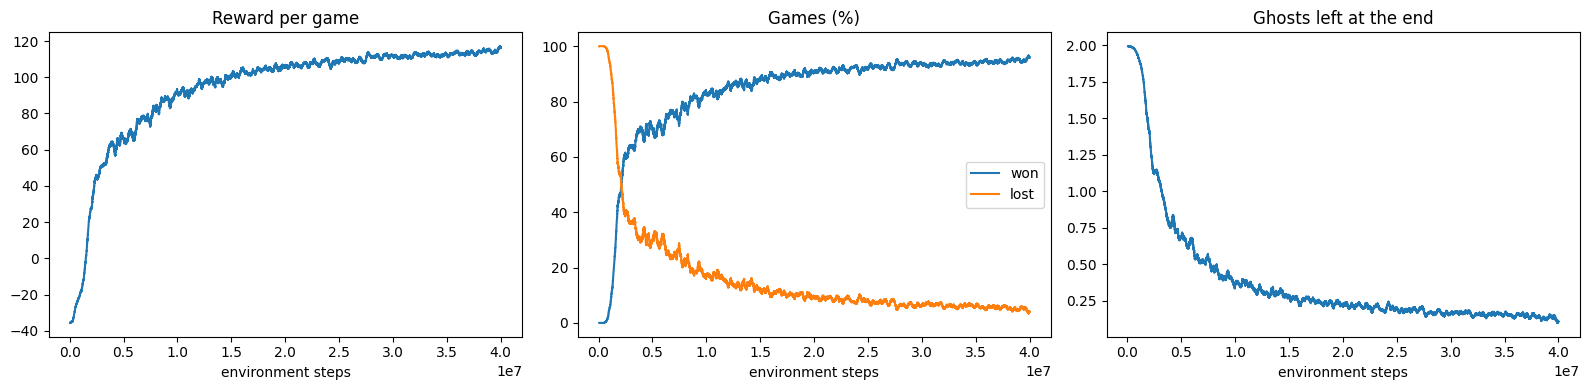
\includegraphics[width=\textwidth]{../Media/a2c_ppo_training.png}
  \caption{Training of the agent \code{Trainings/A2C/PPO\_1} on a Kaggle
    GPU, game \code{v1}: reward per game, games won and lost, and ghosts
    left at the end, against the number of environment steps (averages
    over $2000$ games).}
  \label{fig:ppo-training}
\end{figure}

\begin{pacman}{From $79\%$ to $97\%$}{ppo-results}
  \cref{fig:ppo-training} shows the training of the PPO agent over $40$
  million steps. The agent wins about half of its games after $2$ million
  steps, $80\%$ after $10$ million, and about $95\%$ at the end, while the
  number of ghosts left at the end falls from $2$ to about $0.1$. Evaluated
  on $1000$ games:
  \begin{center}
    \begin{tabular}{@{}lcc@{}}
      \toprule
      & Original A2C & PPO agent (\code{PPO\_1}) \\
      \midrule
      Games won & $79.4\%$ & $96.6\%$ \\
      Games ending with no ghost left & $51.4\%$ & $93.6\%$ \\
      Games with both power cookies eaten & $83.4\%$ & $96.8\%$ \\
      Average number of ghosts left & $0.69$ & $0.095$ \\
      \bottomrule
    \end{tabular}
  \end{center}
  The original A2C agent of the repository used a stride-$2$ network on a
  single RGB image, $n$-step returns and one gradient step per batch. The
  PPO agent differs in several ways at once: feature planes and two
  frames, a full-resolution symmetric network, GAE, PPO updates, a
  curriculum and a larger entropy bonus. Since all were changed together,
  the experiment does not tell how much each one contributes; it shows that
  together they divide the losing rate by six.
\end{pacman}

\section{Summary}

\begin{itemize}[nosep]
  \item The performance difference lemma measures a new policy with the
    advantages of the old one; with importance sampling it gives a
    surrogate objective that can be estimated from the old policy's data
    and agrees with $J$ to first order.
  \item PPO maximises a clipped version of the surrogate, a pessimistic
    bound that removes the incentive to change the probability of an
    action by more than a factor $1 \pm \epsilon$; this allows several
    epochs of mini-batch updates on each batch. A2C is the case of a single
    step.
  \item The KL estimator $(\rho - 1) - \log \rho$ and the clip fraction
    monitor the size of the updates.
  \item On Pacman, PPO with a better input and network wins $96.6\%$ of the
    games, against $79.4\%$ for the original A2C agent.
\end{itemize}
